% !TEX root = ../vr_st.tex

\subsection{Spheres and their wedge sum}\label{ss:Sn}\label{sub:Sn and wedge sum}

For any integer $n \geq 1$ and real number $\rho > 0$, let $\bS^n(\rho)$ be the \defn{$n$-sphere of radius $\rho$}
\[
\bS^n(\rho) = \set{x \in \R^n : \bars{x} = \rho}.
\]
With the induced Riemannian metric, \(\bS^n(\rho)\) is referred to as a \defn{round sphere}.
We simplify notation writing \(\bS^n\) instead of \(\bS^n(1)\).
The constant
\[\zeta_n = \arccos\Big(\frac{-1}{n+1}\Big),\]
which is the diameter of an inscribed regular $(n+1)$-simplex in $\bS^n$, will play an important role.

\subsubsection{}\label{ss:critical values of Sn}

Characterizing the homotopy types of Vietoris--Rips complexes is a challenging question, even for simple spaces like the $n$-spheres. 
For the circle $\bS^1$, a complete answer is provided in \cite{adamaszek2017VietorisProduct}, but for more general spheres $\bS^n$ with $n>1$, only partial results known.

In \cite{adamaszek2018metric}, the authors introduced the Vietoris--Rips metric thickening, a metrization of the Vietoris--Rips complex that embeds the original metric space as a metric subspace. They determined the first scale parameter at which the homotopy type of the thickening of an \(n\)-sphere changes. 
While this does not directly yield the homotopical radius of the \(n\)-sphere, it provides insights into its homotopy behavior and yields homological information, since the thickening shares the same homology as the original Vietoris–Rips complex.

Building on the equivalence between the Kuratowski and Vietoris--Rips filtrations, the authors in \cite{lim2024vietoris} determined both the homotopical radius and the subsequent homotopy type in the Vietoris--Rips filtration of the \(n\)-sphere.

The following lemma is a consequence of these results, along with those from \cite{katz1983filling}.

\lemma
For any $m,n \in \N$ and linear cohomology operation $\theta$ we have:
\begin{enumerate}
	\item \(\crit(\bS^n) = \frac{1}{2}\zeta_n\),
	\item \(\firstdeath{m}{\bS^n} =
	\begin{cases}
		\frac{1}{2}\zeta_n & m = n, \\
		\hfil 0 & m \neq n,
	\end{cases}\)
	\item \(\firstdeath{\theta}{\bS^n} = 0\).
\end{enumerate}

\begin{proof}
	(1) By \cite[Thm.~7.1]{lim2024vietoris}, for any $0 < r \leq \zeta_n$, the space $\VR_r(\bS^n)$ is homotopy equivalent to $\bS^n$, and the homotopy type of $\VR_r(\bS^n)$ changes at $\zeta_n$.
	This implies $\crit(\bS^n)=\frac{1}{2}\zeta_n$.

	\smallskip (2) According to \cite{katz1983filling}, \(\fillrad(\bS^n) = \frac{1}{2}\zeta_n\).
	Applying \cref{ss:beta v.s. fillrad}, we obtain \(\firstdeath{n}{\bS^n} = \frac{1}{2}\zeta_n\).
    When $m\neq n$, the statement follows from the fact that the initial space in the filtration has a trivial degree $m$ reduced homology.

	\smallskip (3) We apply a similar argument as in the $m\neq n$ case of (2). The statement follows from the fact that the initial space in the filtration has trivial $\img_\theta$.
\end{proof}

\subsubsection{}\label{ss:VRSn projection}

Let \(n \in \N\) and \(r \in (0, \zeta_n]\).
From \cite[Thm.~7.1]{lim2024vietoris} we know that the spaces \(\VR_r(\bS^n)\) and \(\bS^n\) have the same homotopy type for any \(n \in \N\).
We now recall from \cite{adamaszek2018metric} a natural map that can be used to realize this equivalence.

In \cite{adamaszek2018metric}, the authors introduced the concept of Vietoris–Rips metric thickenings, which endows the Vietoris–Rips complex with a new topology. 
They define the \defn{canonical projection of \(\VR_r(\bS^n)\)} as the set map 
\[
f_r^n \colon \VR_r(\bS^n) \to \R^{n+1} \setminus \set{0} \to \bS^n,
\]
constructed by first mapping a formal linear combination \(\sum \lambda_i x_i\) to the corresponding point \(\sum \lambda_i x_i\) in \(\mathbb{R}^{n+1}\), followed by a radial projection onto \(\bS^n\). 
Throughout this work, we do not distinguish between a simplicial complex and its geometric realization. 

% We recall the \defn{canonical projection of \(\VR_r(\bS^n)\)}, the map
% \[
% f_r^n \colon \VR_r(\bS^n) \to \R^{n+1} \setminus \set{0} \to \bS^n
% \]
% defined as the composition of the map sending a formal linear combination $\sum\lambda_i x_i$ to the point \(\sum\lambda_i x_i\) in \(\bbR^{n+1}\) and the map sending a point in \(\R^{n+1} \setminus \set{0}\) to its radial projection.
% Here and for the remainder of this work, we do not distinguish between a simplicial complex and its geometric realization.

As mentioned in \cite{adamaszek2018metric}, the map $f_r^n$ is well-defined because, when $r \leq \zeta_n$, the map $\VR_r(\bS^n) \to \R^{n+1}$ misses the origin by the proof of \cite[Lemma 3]{lovasz1983self}. 
Moreover, the authors proved that when \(\VR_r(\bS^n)\) is equipped with the metric thickening topology, the canonical projection is a homotopy equivalence.
  
More recently, \cite{gillespie2024vietoris} showed that the identity map between the Vietoris--Rips complex and the Vietoris--Rips metric thickening is a weak equivalence. 
Consequently, the canonical projection of \(\VR_r(\bS^n)\) is also a weak equivalence for the usual Vietoris--Rips complex. By the Whitehead theorem, this weak equivalence between CW spaces is indeed a homotopy equivalence. 
Thus, the canonical projection remains a homotopy equivalence when \(\VR_r(\bS^n)\) is equipped with the usual topology, as summarized in the following lemma.

\lemma
The canonical projection of the Vietoris--Rips complex \(\VR_r(\bS^n)\) is a homotopy equivalence for every $r \in (0, \zeta_n]$.

% \begin{proof}
%     In \cite{adamaszek2018metric}, a new topology was introduced on the Vietoris--Rips complex, with which the authors proved that the canonical projection of \(\VR_r(\bS^n)\) is a homotopy equivalence.
%     More recently, \cite{gillespie2024vietoris} showed that the identity map is a weak equivalence between this new topology and the usual one.
%     Consequently, the canonical projection of \(\VR_r(\bS^n)\) is a weak equivalence for the usual Vietoris--Rips complex as well.
%     By the Whitehead theorem, this weak equivalence between CW spaces is indeed a homotopy equivalence.
% \end{proof}

\subsubsection{}\label{ss:barcode_Sn}

We apply \cref{ss:critical values of Sn} and the barcode estimates from \cref{ss:barcode_general} to \(\bS^n\).
Using the facts that (1) the reduced homology of \(\bS^n\) has dimension one for \(m = n\) and is zero for all other values of \(m\), and (2) for any linear cohomology operation \(\theta \in \cO(\ell, m)\) with \(\ell \neq m\), \(\img \theta_{\bS^n}\) is trivial, we proceed with the estimation but omit the figure, as it is simply a special case of \cref{fig:barcodes_vs}.

\subsubsection{}\label{ss:barcodes_VS}

For $n \in \N$ and $u_1, \dots, u_n \in \N^n$, let
\[
\VS^{u_1,\dots,u_n} =
\overbrace{\bS^1\vee\dots\vee\bS^1}^{u_1} \vee\dots\vee \overbrace{\bS^n\vee\dots\vee\bS^n}^{u_n}.
\]
Using the homotopy equivalence between the Vietoris--Rips complex of a metric gluing with the wedge sum of the Vietoris--Rips complex described in \cref{ss:wedge sum}, we have the following isomorphisms of persistence modules for \(m \in \N\) and \(\theta \in \cO(\ell,m)\):
\[
\begin{split}
	\rH_m^\VR(\VS^{u_1,\dots,u_n}) &\cong \, \bigoplus_{i=1}^n \rH_m^\VR(\bS^i)^{\oplus u_i}, \\
	\img_\theta^\VR(\VS^{u_1,\dots,u_n}) &\cong \, \bigoplus_{i=1}^n \img_\theta^\VR(\bS^i)^{\oplus u_i}.
\end{split}
\]

Therefore, both the homology barcodes and \(\img_\theta\)-barcodes of \(\VR(\VS^{u_1, \dots, u_n})\) are the multiset unions of the corresponding barcodes of \(\bS^{u_i}\); see \cref{fig:barcodes_vs}.

\begin{figure}
	\centering
	\begin{tikzpicture}[scale=0.52]
	\begin{axis} [
		title = {\LARGE $\Hbarc[\field]{\degp}{\VS^n},1\leq \degp\leq n$},
		ticklabel style = {font=\Large},
		axis y line=middle,
		axis x line=middle,
		ytick={0.5,0.6,0.67,0.95},
		yticklabels={,$\zeta_\degp$,,$\pi$},
		xtick={0.5,0.55,0.95},
		xticklabels={$\frac{\pi}{2}$,$\zeta_n$, $\pi$},
		xmin=-0.015, xmax=1.1,
		ymin=0, ymax=1.1,]
		\addplot [mark=none] coordinates {(0,0) (1,1)};
		\addplot [thick,color=black!20!white,fill=black!30!white,
		fill opacity=0.4]coordinates {
			(0.55,0.95)
			(0.55,0.55)
			(0.95,0.95)
			(0.55,0.95)};
		\addplot [black!40!white,mark=none,dashed, thin] coordinates {(0,0.6) (0.6,0.6)};
		\addplot [black!40!white,mark=none,dashed, thin] coordinates {(0,0.55) (0.55,0.55)};
		\addplot [black!40!white,mark=none,dashed, thin] coordinates {(0.55,0) (0.55,0.55)};
		\addplot[barccolor,mark=*] (0, 0.6) circle (2pt) node[above right,barccolor]{};%{\Large\textsf{1}};
		%\node[mark=none] at (axis cs:0.68,0.21){$\Hbarc{2}{\VS^n}$};
	\end{axis}
\end{tikzpicture}
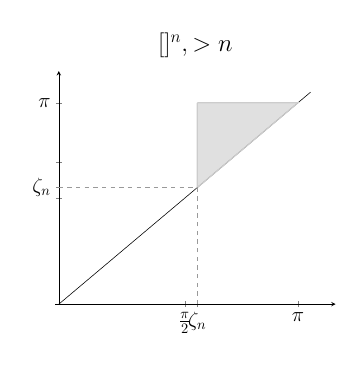
\begin{tikzpicture}[scale=0.52]
	\begin{axis} [
		title = {\LARGE $\Hbarc[\field]{\degp}{\VS^n}, \degp>n$},
		ticklabel style = {font=\Large},
		axis y line=middle,
		axis x line=middle,
		ytick={0.5,0.55,0.67,0.95},
		yticklabels={,$\zeta_n$,,$\pi$},
		xtick={0.5,0.55,0.95},
		xticklabels={$\frac{\pi}{2}$,$\zeta_n$, $\pi$},
		xmin=-0.015, xmax=1.1,
		ymin=0, ymax=1.1,]
		\addplot [mark=none] coordinates {(0,0) (1,1)};
		\addplot [thick,color=black!20!white,fill=black!30!white,
		fill opacity=0.4]coordinates {
			(0.55,0.95)
			(0.55,0.55)
			(0.95,0.95)
			(0.55,0.95)};
		\addplot [black!40!white,mark=none,dashed, thin] coordinates {(0,0.55) (0.55,0.55)};
		\addplot [black!40!white,mark=none,dashed, thin] coordinates {(0.55,0) (0.55,0.55)};
		%\node[mark=none] at (axis cs:0.68,0.21){$\Hbarc[\field]{\degp}{\VS^n}, \degp\geq 3$};
	\end{axis}
\end{tikzpicture}

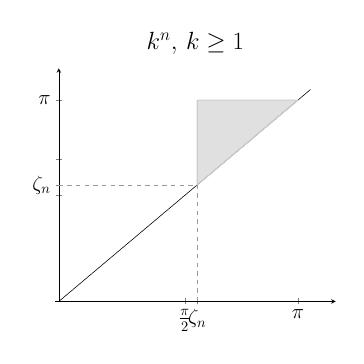
\begin{tikzpicture}[scale=0.52]
	\begin{axis} [
		title={\LARGE $\sqbarc{k}{\VS^n},\, k\geq 1$},
		ticklabel style = {font=\Large},
		axis y line=middle,
		axis x line=middle,
		ytick={0.5,0.55,0.67,0.95},
		yticklabels={,$\zeta_n$,,$\pi$},
		xtick={0.5,0.55,0.95},
		xticklabels={$\frac{\pi}{2}$,$\zeta_n$, $\pi$},
		xmin=-0.015, xmax=1.1,
		ymin=0, ymax=1.1,]
		\addplot [mark=none] coordinates {(0,0) (1,1)};
		\addplot [thick,color=black!20!white,fill=black!30!white,
		fill opacity=0.4]coordinates {
			(0.55,0.95)
			(0.55,0.55)
			(0.95,0.95)
			(0.55,0.95)};
		\addplot [black!40!white,mark=none,dashed, thin] coordinates {(0,0.55) (0.55,0.55)};
		\addplot [black!40!white,mark=none,dashed, thin] coordinates {(0.55,0) (0.55,0.55)};
		%\node[mark=none] at (axis cs:0.68,0.21){$\sqbarc{k}{\VS^n},\, k\geq 1$};
	\end{axis}
\end{tikzpicture}

	\caption{Let $\VS = \VS^{u_1,\dots,u_n}$ for some tuple of non-negative integers.
		\emph{Top row:} persistent reduced homology barcodes of $\VS$, where the dot $(0,\zeta_m)$ has multiplicity $u_m$ which can be zero.
		\emph{Bottom row:} $\img_\theta$-barcodes of $\VS$ where $\theta \in \cO(\ell,m)$ with \(\ell \neq m\).
        In each figure, the gray region represents where additional bars could exist within the corresponding barcode.
        See \cref{ss:barcode_Sn} for the case when the wedge sum is a single sphere and see \cref{ss:barcodes_VS} for the general case.}
	\label{fig:barcodes_vs}
\end{figure}